\documentclass[11pt,a4paper]{article}

% --- Essential Packages ---
\usepackage[utf8]{inputenc}
\usepackage[T1]{fontenc}
\usepackage{lmodern}
\usepackage[margin=2.5cm]{geometry}
\usepackage{amsmath,amssymb}
\usepackage{graphicx}
\usepackage{booktabs}
\usepackage{tabularx}
\usepackage{xcolor}
\usepackage{fancyhdr}
\usepackage{titlesec}
\usepackage{enumitem}
\usepackage{caption}
\usepackage{tikz}
\usetikzlibrary{shapes.geometric, arrows.meta, positioning}

% --- Color Palette ---
\definecolor{primary}{RGB}{35, 45, 65}       % Deep Navy
\definecolor{accent}{RGB}{41, 128, 185}      % Blue
\definecolor{darkgray}{RGB}{70, 70, 70}
\definecolor{lightgray}{RGB}{245, 245, 248}
\definecolor{boxborder}{RGB}{190, 195, 205}

% --- Hyperlinks ---
\usepackage{hyperref}
\hypersetup{
    colorlinks=true,
    linkcolor=accent,
    filecolor=primary,
    urlcolor=accent
}

% --- Header and Footer ---
\pagestyle{fancy}
\fancyhf{}
\fancyhead[L]{\small \textcolor{darkgray}{Pixel Adventure — Game Design Document}}
\fancyhead[R]{\small \textcolor{darkgray}{Lean GDD}}
\fancyfoot[L]{\small \textcolor{darkgray}{Student: Ahmed Amin Al-Hindwan}}
\fancyfoot[R]{\thepage}
\renewcommand{\headrulewidth}{0.4pt}
\renewcommand{\footrulewidth}{0.4pt}

% --- Section Styling ---
\titleformat{\section}{\large\bfseries\color{primary}}{\thesection}{0.8em}{}[\titlerule]
\titleformat{\subsection}{\normalsize\bfseries\color{accent}}{\thesubsection}{0.6em}{}

% --- Simple Flowchart / Diagram Styles ---
\tikzstyle{nodebox} = [rectangle, rounded corners=4pt, draw=primary, fill=lightgray, text centered, minimum height=0.7cm, minimum width=2.4cm, font=\small]
\tikzstyle{startbox} = [rectangle, rounded corners=10pt, draw=primary, fill=primary!15, text centered, minimum height=0.7cm, minimum width=2.5cm, font=\small\bfseries]
\tikzstyle{decision} = [diamond, aspect=1.8, draw=accent, fill=accent!15, text centered, font=\footnotesize]
\tikzstyle{link} = [thick, -Stealth, color=primary]

% --- Simple Screenshot Box ---
\newcommand{\screenshot}[2]{%
\begin{figure}[htbp]
    \centering
    \IfFileExists{#1}{%
        \includegraphics[width=0.8\textwidth, height=5.5cm, keepaspectratio]{#1}%
    }{%
        \setlength{\fboxsep}{10pt}%
        \fbox{%
            \begin{minipage}[c][4.5cm][c]{0.78\textwidth}
                \centering
                {\large\bfseries\color{primary} #2}\par\vspace{0.3cm}
                {\small\color{darkgray} [ Screenshot Placeholder: \texttt{\detokenize{#1}} ]}\par\vspace{0.2cm}
                {\footnotesize\itshape Resolution: 640 $\times$ 360 px}
            \end{minipage}%
        }%
    }
    \caption{#2}
    \label{fig:\detokenize{#1}}
\end{figure}
}

\begin{document}

% =========================================================================
% TITLE PAGE
% =========================================================================
\begin{titlepage}
    \centering
    \vspace*{2cm}
    
    {\LARGE \bfseries \color{primary} Pixel Adventure}\\[0.3cm]
    {\large \bfseries \color{accent} 2D Pixel-Art Platformer Game}\\[0.6cm]
    {\normalsize Lean Indie Game Design Document (GDD)}\\[2.5cm]
    
    \begin{minipage}{0.8\textwidth}
        \centering \small \color{darkgray}
        A concise, practical game design and systems document describing the core mechanics, gameplay flow, and architecture of the \textbf{Pixel Adventure} project built with \textbf{Flutter} and \textbf{Flame Engine}.
    \end{minipage}
    
    \vfill
    
    \begin{minipage}{0.45\textwidth}
        \begin{flushleft}
            \textbf{\color{primary} Student / Author:}\\
            Ahmed Amin Al-Hindwan
        \end{flushleft}
    \end{minipage}
    \hfill
    \begin{minipage}{0.45\textwidth}
        \begin{flushright}
            \textbf{\color{primary} Supervisor / Instructor:}\\
            Salem Al-Soumhi
        \end{flushright}
    \end{minipage}
    
    \vspace{2cm}
    {\footnotesize Engine: Flutter / Flame Engine \quad | \quad Viewport: 640 $\times$ 360 px \quad | \quad Date: \today}
    \vspace*{1cm}
\end{titlepage}

\tableofcontents
\newpage

% =========================================================================
% 1. INTRODUCTION
% =========================================================================
\section{Introduction}

\subsection{Project Overview}
\textbf{Pixel Adventure} is a 2D indie platformer game developed in \textbf{Flutter} using the \textbf{Flame} engine. It features retro pixel-art visuals, tile-based levels designed in Tiled, multi-frame character animations, and smooth physics-based movement.

\subsection{Core Concept}
The player controls an agile hero (\textit{Mask Dude}) through a 2D level filled with moving hazards, enemy patrols, and collectible items. The player's main goal is to safely reach the end checkpoint to clear the stage and unlock the next level.

\subsection{Core Gameplay Loop}
The gameplay loop consists of four direct steps:
\begin{enumerate}[noitemsep]
    \item \textbf{Spawn:} The player starts at the level's entry point.
    \item \textbf{Platforming:} Move and jump across solid ground and floating platforms.
    \item \textbf{Action \& Interaction:}
    \begin{itemize}[noitemsep]
        \item Collect fruit items for score and audio feedback.
        \item Avoid moving saws and enemy flanks (which trigger an instant respawn).
        \item Jump onto enemies from above to defeat them and bounce upward.
    \end{itemize}
    \item \textbf{Level Goal:} Reach the checkpoint post to raise the flag and progress to the next stage.
\end{enumerate}

% =========================================================================
% 2. OBJECTIVES
% =========================================================================
\section{Objectives}

\subsection{Technical Objectives}
\begin{itemize}[noitemsep]
    \item \textbf{Component-Based Structure:} Build game entities (Player, Enemies, Traps, Items) as modular Flame components.
    \item \textbf{Smooth 2D Physics:} Implement standard gravity, variable jump velocity, and solid platform collision checks.
    \item \textbf{Tilemap Loading:} Read levels and object coordinates dynamically from TMX files.
    \item \textbf{Dual Controls:} Support keyboard inputs for desktop and touch screen controls (Virtual Joystick and Jump Button) for mobile.
    \item \textbf{Audio Feedback:} Trigger non-blocking sound effects for jumps, pickups, hits, and level clears.
\end{itemize}

\subsection{Player Objectives}
\begin{itemize}[noitemsep]
    \item \textbf{Win Condition:} Reach the checkpoint flag to finish the level.
    \item \textbf{Collection:} Collect all fruits scattered across the map.
    \item \textbf{Survival:} Avoid touching moving saw blades.
    \item \textbf{Combat:} Stomp patrol chickens by landing on their heads from above.
    \item \textbf{Respawn Rule:} Taking a hit from a trap or enemy flank instantly respawns the player at the start point.
\end{itemize}

% =========================================================================
% 3. USE CASES
% =========================================================================
\section{Use Cases}

\subsection{Use Case Table}
Table~\ref{tab:usecases} outlines the actual player and system actions implemented in the code.

\begin{table}[htbp]
\centering
\small
\caption{Core Game Use Cases}
\label{tab:usecases}
\begin{tabularx}{\textwidth}{l p{3.2cm} p{2.2cm} X}
\toprule
\textbf{ID} & \textbf{Use Case} & \textbf{Actor} & \textbf{Main Action / Flow} \\
\midrule
\textbf{UC-01} & Move Horizontally & Player & Press Left/Right or tilt Joystick $\rightarrow$ Character moves and flips direction. \\
\midrule
\textbf{UC-02} & Jump & Player & Press Space or tap Jump Button $\rightarrow$ Character jumps with sound effect. \\
\midrule
\textbf{UC-03} & Collect Fruit & Player & Touch Fruit item $\rightarrow$ Play pickup sound, play burst animation, remove fruit. \\
\midrule
\textbf{UC-04} & Stomp Enemy & Player & Land on Chicken from above $\rightarrow$ Enemy defeated, player bounces upward. \\
\midrule
\textbf{UC-05} & Hit Hazard / Respawn & Player & Touch Saw or touch enemy from the side $\rightarrow$ Play hit sound and respawn at start. \\
\midrule
\textbf{UC-06} & Reach Checkpoint & Player & Touch Checkpoint $\rightarrow$ Flag raises, exit animation plays, next level loads. \\
\bottomrule
\end{tabularx}
\end{table}

\subsection{Use Case Diagram}
Figure~\ref{fig:usecasediagram} illustrates the player and game system interactions.

\begin{figure}[htbp]
\centering
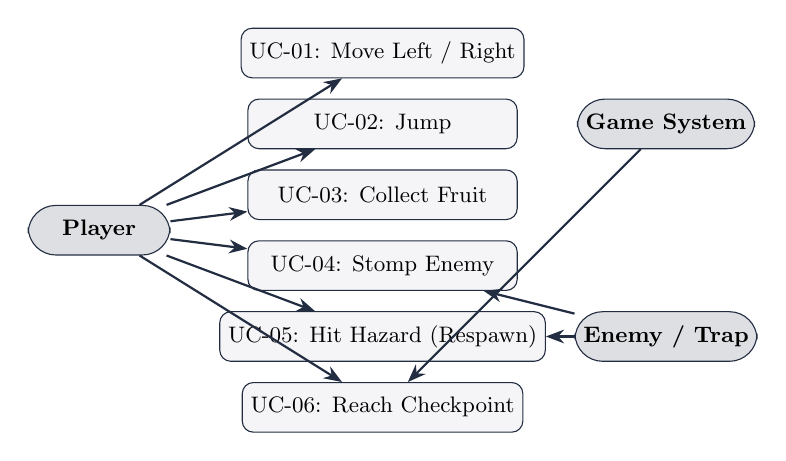
\begin{tikzpicture}[scale=0.9, every node/.style={transform shape}]
    % Actors
    \node[startbox, minimum width=2cm] (player) at (-4, 0) {Player};
    \node[startbox, minimum width=2cm] (enemy)  at (4, -1.5) {Enemy / Trap};
    \node[startbox, minimum width=2cm] (game)   at (4, 1.5) {Game System};

    % Use Cases
    \node[nodebox, minimum width=3.8cm] (uc1) at (0, 2.5) {UC-01: Move Left / Right};
    \node[nodebox, minimum width=3.8cm] (uc2) at (0, 1.5) {UC-02: Jump};
    \node[nodebox, minimum width=3.8cm] (uc3) at (0, 0.5) {UC-03: Collect Fruit};
    \node[nodebox, minimum width=3.8cm] (uc4) at (0, -0.5) {UC-04: Stomp Enemy};
    \node[nodebox, minimum width=3.8cm] (uc5) at (0, -1.5) {UC-05: Hit Hazard (Respawn)};
    \node[nodebox, minimum width=3.8cm] (uc6) at (0, -2.5) {UC-06: Reach Checkpoint};

    % Connections
    \draw[link] (player) -- (uc1);
    \draw[link] (player) -- (uc2);
    \draw[link] (player) -- (uc3);
    \draw[link] (player) -- (uc4);
    \draw[link] (player) -- (uc5);
    \draw[link] (player) -- (uc6);

    \draw[link] (enemy) -- (uc4);
    \draw[link] (enemy) -- (uc5);
    \draw[link] (game)  -- (uc6);
\end{tikzpicture}
\caption{System Use Case Diagram.}
\label{fig:usecasediagram}
\end{figure}

\newpage
% =========================================================================
% 4. GAME LOGIC FLOWCHART
% =========================================================================
\section{Game Logic Flowchart}

Figure~\ref{fig:flowchart} shows the clear, simplified lifecycle of the game from launch to victory or respawn.

\begin{figure}[htbp]
\centering
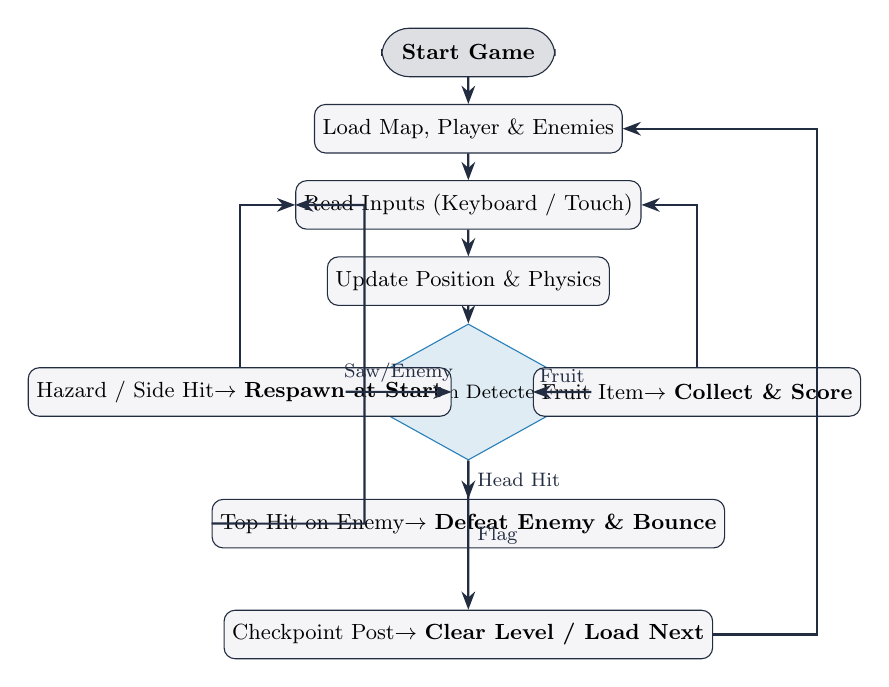
\begin{tikzpicture}[node distance=1.1cm and 1.8cm, auto, scale=0.88, every node/.style={transform shape}]
    % Flow Nodes
    \node[startbox] (start) {Start Game};
    \node[nodebox, below of=start] (load) {Load Map, Player \& Enemies};
    \node[nodebox, below of=load] (loop) {Read Inputs (Keyboard / Touch)};
    \node[nodebox, below of=loop] (move) {Update Position \& Physics};
    \node[decision, below of=move, yshift=-0.5cm] (col) {Collision Detected?};

    % Branch Outcomes
    \node[nodebox, left of=col, xshift=-2.2cm] (respawn) {Hazard / Side Hit\\$\rightarrow$ \textbf{Respawn at Start}};
    \node[nodebox, below of=col, yshift=-0.8cm] (stomp) {Top Hit on Enemy\\$\rightarrow$ \textbf{Defeat Enemy \& Bounce}};
    \node[nodebox, right of=col, xshift=2.2cm] (fruit) {Fruit Item\\$\rightarrow$ \textbf{Collect \& Score}};
    \node[nodebox, below of=stomp, yshift=-0.5cm] (goal) {Checkpoint Post\\$\rightarrow$ \textbf{Clear Level / Load Next}};

    % Connecting lines
    \draw[link] (start) -- (load);
    \draw[link] (load) -- (loop);
    \draw[link] (loop) -- (move);
    \draw[link] (move) -- (col);

    \draw[link] (col) -- node[above] {\footnotesize Saw/Enemy} (respawn);
    \draw[link] (col) -- node[right] {\footnotesize Head Hit} (stomp);
    \draw[link] (col) -- node[above] {\footnotesize Fruit} (fruit);
    \draw[link] (col) -- node[right] {\footnotesize Flag} (goal);

    % Return paths
    \draw[link] (respawn) |- (loop);
    \draw[link] (stomp)   -- ++(-1.5,0) |- (loop);
    \draw[link] (fruit)   |- (loop);
    \draw[link] (goal.east) -- ++(1.5,0) |- (load);
\end{tikzpicture}
\caption{Simplified Game Logic Flowchart.}
\label{fig:flowchart}
\end{figure}

% =========================================================================
% 5. USER INTERFACES (UI/UX)
% =========================================================================
\section{User Interfaces (UI/UX)}

\subsection{In-Game Viewport and Controls}
\begin{itemize}[noitemsep]
    \item \textbf{Game Viewport:} Fixed $640 \times 360$ landscape camera with an auto-scrolling parallax background.
    \item \textbf{Virtual Joystick (Bottom-Left):} On-screen touch stick for moving left and right on mobile devices.
    \item \textbf{Jump Button (Bottom-Right):} On-screen button for jump actions on mobile devices.
\end{itemize}

\subsection{Screenshot Placeholders}
The following boxes are reserved for actual game screenshots:

\screenshot{screenshots/gameplay-level-01.png}{Main Gameplay Screen (Level-01 Platforming)}

\screenshot{screenshots/hud-controls-overlay.png}{Virtual Touch HUD Controls (Joystick and Jump Button)}

\screenshot{screenshots/checkpoint-activation.png}{Checkpoint Goal Reached (Level Clear)}

\screenshot{screenshots/chicken-stomp-encounter.png}{Enemy Interaction (Jump Stomp Bounce)}

\subsection{Menu Assets in Project}
The project repository contains pixel-art UI button sprites ready in \texttt{assets/images/Menu/}:
\begin{itemize}[noitemsep]
    \item \textbf{Play Button:} For starting the game from a main menu.
    \item \textbf{Settings \& Volume Buttons:} For sound and audio control screens.
    \item \textbf{Restart \& Back Buttons:} For in-game pause and level retry dialogs.
    \item \textbf{Level Select Badges (01 to 50):} For a future stage selection screen.
\end{itemize}

% =========================================================================
% 6. FUTURE ENHANCEMENTS
% =========================================================================
\section{Future Enhancements}

\begin{enumerate}
    \item \textbf{Save System:} Store player progress, collected fruits, and unlocked levels locally on the device.
    \item \textbf{Add More Levels:} Link \texttt{Level-02.tmx} (already present in the assets folder) into the active level list.
    \item \textbf{Main Menu \& Pause Overlay:} Build a clean Start Menu and Pause Screen using the available button assets.
    \item \textbf{More Enemies and Traps:} Add additional enemy types (like \textit{Angry Pig} and \textit{Bat}) and traps (like \textit{Spikes}) already available in the project sprites.
    \item \textbf{Health / Lives System:} Introduce a 3-heart health system so the player gets a Game Over screen instead of infinite respawns.
    \item \textbf{Background Music (BGM):} Add looping background music tracks alongside the existing sound effects.
\end{enumerate}

\end{document}
